\documentclass[a4paper]{article}
\usepackage[a4paper]{geometry}
\usepackage{amsmath}
\usepackage{amssymb}
\usepackage[utf8]{inputenc}
\usepackage{graphicx}
\usepackage{booktabs}
\usepackage[russian]{babel}
\usepackage{flafter}
\usepackage{caption}

\title{Лабораторная работа 2.5.1 \\Измерение коэффициента поверхностного натяжения жидкости}
\date{02 апреля 2017 г.}
\author{Вячеслав Ждановский, студент 611 группы ФРКТ\\
Шамиль Вагабов, студент 611 группы ФРКТ\\
Станислав Токарев, студент 611 группы ФРКТ\\
Кичин Егор, студент 611 группы ФРКТ}
\begin{document}	
\pagenumbering{gobble}
	\maketitle
	\newpage
	\pagenumbering{arabic}
	
	\paragraph{Цель работы:} 1) измерение коэффициента поверхностного натяжения исследуемой жидкости при разной температуре с использованием известного коэффициента поверхностного натяжения другой жидкости; 2) определние полной поверхностной энергии и теплоты, необходимой для изотермического образования единицы поверхности жидкости.
	\paragraph{В работе используются:}прибор Ребиндера с термостатом; исследуемые жидкости; стаканы.
	\section{Теория}
	Наличие поверхностного слоя приводит к различию давлений по разные стороны от искривлённой границы раздела двух сред. Для сферического пузырька внутри жидкости избыточное давление дается формулой Лапласа:
	\begin{equation}
	\Delta P = P_\text{внутри} - P_\text{снаружи}=\frac{2\sigma}{r}.
	\end{equation}
	Эта формула лежит в основе предлагаемого метода определения коэффициента поверхностного натяжение жидкости. Измеряется давления, необходимое для выталкивания в жидкость пузырька газа.
	\section{Экспериментальная установка}
	\begin{figure}[ht!]
		\centering
		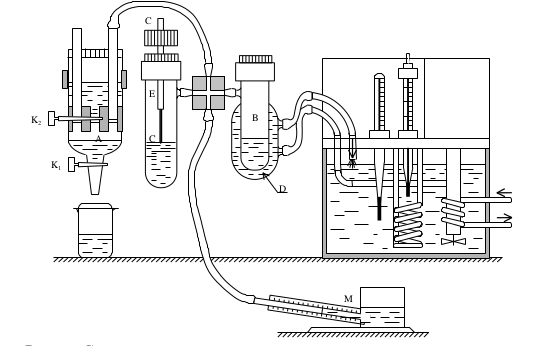
\includegraphics[height=80mm]{pic1.png}
		\caption{Схема экспериментальной установки. A, B, E - сосуды. C - полая металлическая игла. К$_1$, K$_2$ - краны. М - манометр. А - аспиратор. \label{overflow}}
	\end{figure}
	\section{Ход работы}
	1. Убеждаемся в исправности установки. Устанавливаем иглу так, чтобы её кончик лишь коснулся поверхности воды. Установив скорость падения капель примерно 1 капля в 5 секунд, добъемся пробулькивания пузырьков и того, что манометр показывает медленный рост давления до некоторого максимального значения и затем быстрое его падения при пробулькивания пузырька. \\ 
	2. Устанавливаем достаточно малую частоту падения капель - максимальное давление не зависит от этой частоты. \\
	3. Измерим максимальное значение при пробулькивании пузырька. При этом заметного разброса вне систематической погрешности манометра не наблюдалось.  \\
	\begin{equation}
	P_{max} = 40 \cdot 0.2 \cdot 9.8 = 78.4\text{ Па}
	\end{equation}
	4. Найдем из (1) диаметр иглы.
	\begin{equation}
	d=\frac{4\sigma}{\Delta P}=1.16 \pm 0.03\text{ мм}
	\end{equation}
	Сравненим полученное значение с прямыми измерениями:
	\begin{equation}
	d_\text{прям}=1.10 \pm 0.05 \text{ мм}
	\end{equation}
	Заметим, что результат попал в диапазон погрешности измерений. \\
	5. Перенесем иглу в сосуд с анилином (при этом не забыв ее вытереть). \\
	6. Измерим максимальное давление в пузырьках, когда игла лишь касается поверхности жидкости.
	\begin{equation}
	P_1=235 \pm 2 \text{ Па}
	\end{equation}
	Измерим максимальное давление, когда игла почти полностью утоплена.
	\begin{equation}
	P_2=302 \pm 2 \text{ Па}
	\end{equation}
	Измерим $\Delta$h линейкой:
	\begin{equation}
	\Delta h_\text{прям}=7 \pm 1 \text{мм}
	\end{equation}
	Найдем $\Delta$h по косвенным измерениям:
	\begin{equation}
	\Delta h_\text{прям}=\frac{\Delta P}{\rho g}=\frac{302-235}{1026\cdot 9.8}=6.6 \pm 0.3 \text{мм}
	\end{equation}
	Снова убеждаемся в попадании в диапазон погрешности. \\
	7. Снимем зависимость $\sigma (T)$ при нагревании анилина при помощи термостата. \\
	\begin{table}[h!]
 		\centering
	\begin{tabular}{|c|c|c|c|c|c|c|}
	\hline
t, $^o$C & 24 & 29 & 33 & 37 & 41 & 45 \\
\hline
$\Delta$P, Па& 77&	74&	72&	67&	64&	61	\\
\hline
$\sigma$, $10^{-3} \frac{\text{Н}}{\text{м}^3}$ & 42.4 & 40.7 &	39.6& 36.9 & 35.2 & 33.6 \\
\hline
    	\end{tabular}
  		\caption{Измерения зависимости $\sigma$ от T}
	\end{table}
	\begin{figure}[ht!]
		\centering
		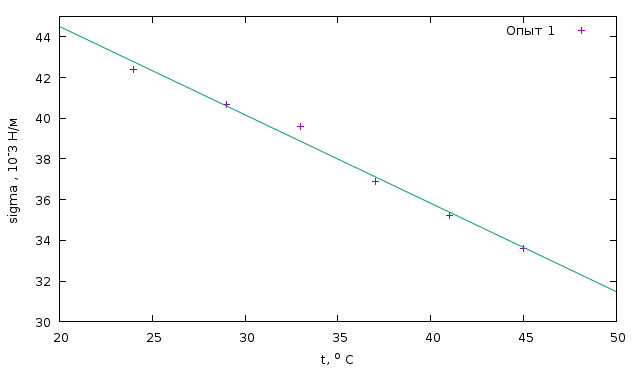
\includegraphics[height=80mm]{pic2.png}
		\caption{Полученный график \label{overflow}}
	\end{figure}
	\\8. Из графика находим:
	\begin{equation}
	\frac{d\sigma}{dT}=-0.43 \pm 0.02 \text{ }\frac{\text{Н}}{\text{м}^3\text{К}}
	\end{equation}
	\section{Авторы} Вячеслав Ждановский, студент 611 группы ФРКТ\\
Шамиль Вагабов, студент 611 группы ФРКТ\\
Станислав Токарев, студент 611 группы ФРКТ\\
Кичин Егор, студент 611 группы ФРКТ
\end{document}